
\subsection{Experiments description}
In this section we compare the decomposition algorithm (both with Armijo and exact line search) against SNOPT \cite{snopt}.
The decomposition algorithm is written in \textit{Python 2.7} while we use the official Python interface for SNOPT. We also use \texttt{numpy} library, linked with \texttt{blas} and \texttt{ATLAS} libraries. The PC used for the experiments is equipped with and Intel i7 3630QM processor, 8GB of RAM and a Linux based distribution.\\
In order to obtain comparable results, in our scheme we use a \textit{stop criterion} that is the same used by SNOPT, i.e. we stop the algorithm when
\begin{equation}
\left| \frac{\partial f(x^k,y^k)}{d{x_{j(k)}}} - \frac{\partial f(x^k,y^k)}{d{x_{i(k)}} }\right| < \epsilon
\end{equation}
In SNOPT, this is (almost) equivalent to set the \texttt{Major optimality tolerance} optional parameter to $\epsilon$. 
In all the following experiments we used the NASDAQ-2196 dataset\footnotemark[1]; from the covariance matrix contained in the dataset, we compute the correlation matrix and we use that instead of the covariance one for numerical reasons. In our experiments we set $l = [0,..,0] \in \mathbb{R}^n$ and  $u = [1,..,1] \in \mathbb{R}^n$ except in section (\ref{bounded}) where we use different box constraints.
\footnotetext[1]{NASDAQ-2196 dataset can be downloaded at \url{http://host.uniroma3.it/docenti/cesarone/datasetsw3_tardella.html}}

\subsection{Execution time}
In Figure (\ref{fig:perf}) we compare the average execution time of the decomposition algorithm (with inexact and exact line search) against SNOPT. \textit{TODO: inserire commenti}
\begin{figure}
\makebox[\textwidth][c]{
\begin{tikzpicture}
\begin{axis}[%
xlabel={\# of assets},
ylabel={Exe Time (s)},
legend pos=north west
]
\addplot [color=blue,solid,mark=x,mark options={solid}]
  table[row sep=crcr]{%
100	.148\\
200	.346	\\
300	.583	\\
500	1.486	\\
750	3.147		\\
1000 6.431 \\
1250 11.57 \\
1500 18.6\\
};
\label{Subplot:exe_e6_exact}

\addplot [color=red,solid,mark=x,mark options={solid}]
  table[row sep=crcr]{%
100	 .101   \\
200	 .269	\\
300	 .481	\\
500	 1.417	\\
750	 3.763	\\
1000 8.72  \\
1250 17.16 \\
1500 28.75 \\
};
\label{Subplot:exe_e6_armijo}

\addplot [color=gr,solid,mark=x,mark options={solid}]
  table[row sep=crcr]{%
100	.008		\\
200	.028		\\
300	.074	    \\
500	.353	    \\
750	 1.197  \\
1000 3.15	\\
1250 6.617	\\
1500 11.765 \\
};
\label{Subplot:exe_e6_snopt}
\addlegendentry{Exact LS}
\addlegendentry{Armijo LS}
\addlegendentry{SNOPT}
\end{axis}
\end{tikzpicture}
}
\caption{Comparison of average execution time with {$\epsilon=10^{-10}$} on the NASDAQ-2196 dataset}
\label{fig:perf}
\end{figure}


\subsection{Iterations}
In Figure (\ref{fig:it}) we compare the average number of iterations performed by the decomposition algorithm using the two different strategies for step computation (inexact and exact). \textit{TODO: inserire commenti}
\begin{figure}
\makebox[\textwidth][c]{
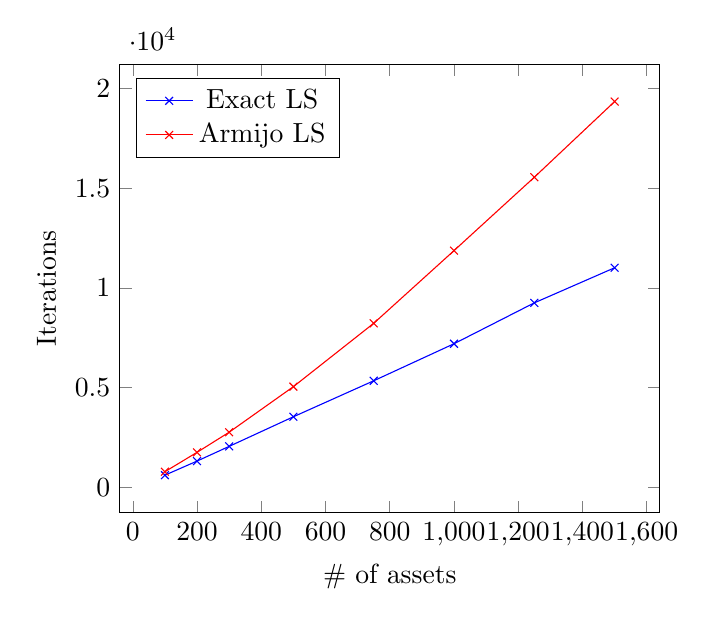
\begin{tikzpicture}
\begin{axis}[%
xlabel={\# of assets},
ylabel={Iterations},
legend pos=north west
]
\addplot [color=blue,solid,mark=x,mark options={solid}]
  table[row sep=crcr]{%
%50	242\\
%75	379\\
100	609 \\
200	1315 \\
300	2053 \\
500	3538\\
750	5343 \\
1000	7200\\
1250	9251\\
1500    11011\\
};

\addplot [color=red,solid,mark=x,mark options={solid}]
 table[row sep=crcr]{%
%%50	309    \\
%%75	483    \\
100	782    \\
200	1754		\\
300	2763		\\
500	5048		\\
750	8225		\\
1000	 11871	\\
1250	 15552	\\
1500	 19347\\
};

\addlegendentry{Exact LS}
\addlegendentry{Armijo LS}
\end{axis}
\end{tikzpicture}
}
\caption{Comparison of average number of iterations performed to converge with {$\epsilon=10^{-10}$} on the NASDAQ-2196 dataset}
\label{fig:it}
\end{figure}

\subsection{Convergence to a Risk Parity solution}
In this section we evaluate the probability to converge to a critical point $(x^*,y^*)$ that is also a Risk Parity solution, i.e. that satisfies 
\begin{equation}\label{eq:reseps}
\max_i \left| \frac{RC_i}{\mathcal{R}(x^*,y^*)} - \frac{1}{n} \right| < 10^{-6}
\end{equation}
where $RC_i$ is the risk contribution of the asset $i$ and ${\mathcal{R}(x^*,y^*)}$ is the total risk of the invested portfolio. Equation (\ref{eq:reseps}) express the fact that the (normalized) max deviation from Risk Parity of the solutions is less than $10^{-6}$. In Table (\ref{tab:first}) and (\ref{tab:second}) we compare the probability to reach a Risk Parity solution for both the decomposition algorithm (with inexact and exact line search) and SNOPT, using different choices of the starting point $x^0$. In Figure (\ref{fig:sparsity}) we measure the probability to reach a Risk Parity solution varying the sparsity of the initial guess $x^0$, i.e. the percentage of components of $x^0$ fixed to 0. \textit{TODO: inserire commenti}
\begin{table}
\centering
\begin{tabular}{ c | c | c | c }
n &  G-S$_{(ALS)}$ & G-S$_{(ELS)}$  & SNOPT \\\hline
5    & 100.0\% & 100.0\% & 100.0\%\\\hline
10   & 100.0\% & 100.0\% & 100.0\%\\\hline
20   & 100.0\% & 100.0\% & 100.0\%\\\hline
50   & 99.0\%  & 99.4\%  & 99.5\%\\\hline
100  & 85.4\%  & 87.0\%  & 91.2\%\\\hline
200  & 40.0\%  & 45.0\%  & 52.0\%\\\hline
300  & 22.0\%  & 24.0\%  & 34.0\%\\\hline
500  & 0.0\%   & 6.0\%   & 3.0\%\\\hline
750  & 0.0\%   & 2.0\%   & 0.0\%\\\hline
1000 & 0.0\%   & 0.0\%   & 0.0\%\\\hline
1250 & 0.0\%   & 0.0\%   & 0.0\%\\\hline
\end{tabular}
\caption{Probability to converge to a Risk Parity solution using $x^{0}_i = 1/n \quad \forall i$}
\label{tab:first}
\end{table}


\begin{table}
\centering
\begin{tabular}{ c | c | c | c}
n &  G-S$_{(ALS)}$ & G-S$_{(ELS)}$  & SNOPT \\\hline
5    & 100.0\%  & 100.0\% & 100.0\%\\\hline
10   & 100.0\%  & 100.0\% & 99.9\%\\\hline
20   & 100.0\%  & 100.0\%  & 100.0\%\\\hline
50   & 100.0\%  & 99.9\%  & 99.9\%\\\hline
100  & 99.9\%   & 100.0\%  & 99.6\% \\\hline
200  & 100.0\%  & 100.0\%  & 98.8\% \\\hline
300  & 100.0\%  & 100.0\%  & 96.6\% \\\hline
500  & 99.5\%   & 99.2\%   & 88.0\%\\\hline
750  & 99.5\%   & 99.2\%  & 83.0\%\\\hline
1000 & 98.0\%   & 95.2\%  & 83.0\%\\\hline
1250 & 91.5\%   & 93.2\%  & 73.0\%\\\hline
\end{tabular}
\caption{Probability to converge to a Risk Parity solution using $x^{0}= [1, 0, .., 0]$}
\label{tab:second}
\end{table}

\begin{figure}
\begin{center}
\makebox[0.5\textwidth][c]{
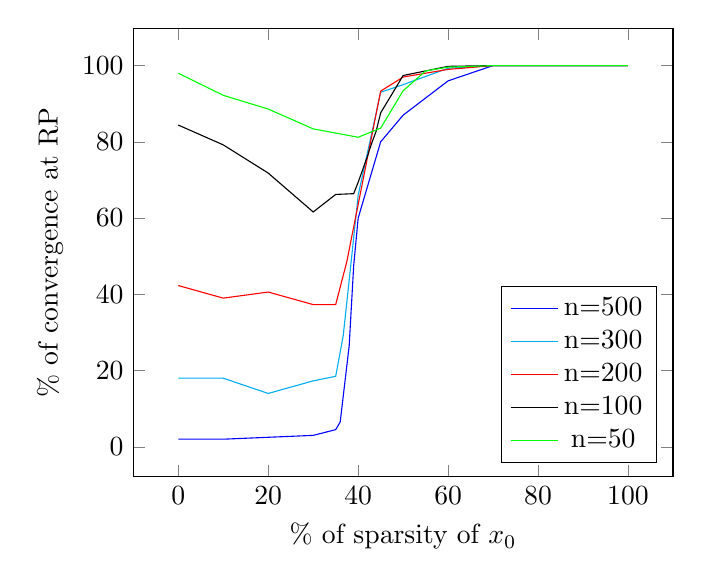
\begin{tikzpicture}
\begin{axis}[%
xlabel={\% of sparsity of $x_0$},
ylabel={\% of convergence at RP},
scaled y ticks=false,
legend pos=south east
]

\addplot [color=blue,solid,mark=none,mark options={solid}]
  table[row sep=crcr]{%
0 2 \\
10 2 \\
20 2.5 \\
30 3 \\
35 4.5 \\
36 6.5
37 14.5 \\
38 26.5 \\
39 47.5 \\
40 60 \\
45 80\\
50 87 \\
60 96 \\
70 100 \\
80 100 \\
90 100 \\
100 100 \\
};

\addplot [color=cyan,solid,mark=none,mark options={solid}]
  table[row sep=crcr]{%
0 18\\
10 18 \\
20 14 \\
30 17.3 \\
35 18.5 \\
36.67 29.1 \\
38.3 47 \\
40 66 \\
45 93 \\
50 95 \\
60 99.3 \\
70 100 \\
80 100 \\
90 100 \\
100 100\\
};

\addplot [color=red,solid,mark=none,mark options={solid}]
  table[row sep=crcr]{%
0 42.3 \\
10 39 \\
20 40.6 \\
30 37.3 \\
35 37.3 \\
37.5 48.7 \\
38.5 54.7 \\
40 63.6 \\
45 93.3 \\
50 97 \\
60 99 \\
70 100 \\
80 100 \\
90 100 \\
100 100\\
};

\addplot [color=black,solid,mark=none,mark options={solid}]
  table[row sep=crcr]{%
0 84.4 \\
10 79.2 \\
20 71.8 \\
30 61.6 \\
35 66.2 \\
39 66.4 \\
40 69.4 \\
42 76 \\
43 79.6 \\
44 82.8\\
45 87.6 \\
50 97.4 \\
60 99.8 \\
70 100 \\
80 100 \\
90 100 \\
100 100\\
};

\addplot [color=green,solid,mark=none,mark options={solid}]
  table[row sep=crcr]{%
0 98 \\
10 92.2 \\
20 88.6\\
30 83.4 \\
40 81.2 \\
45 83.6 \\
50 93.4 \\
55 98.6 \\
60 99.6 \\
70 100 \\
80 100 \\
90 100 \\
100 100 \\
};
\addlegendentry{n=500}
\addlegendentry{n=300}
\addlegendentry{n=200}
\addlegendentry{n=100}
\addlegendentry{n=50}
\end{axis}

\end{tikzpicture}
}
\end{center}

\caption{\% of computations that find an RP solution, varying the sparsity of the initial guess $x^0$, for different number of assets $n$}
\label{fig:sparsity}
\end{figure}

\subsection{Bounds on assets}\label{bounded}
In this section we use different combinations for the box constraints $l$ and $u$ and we compare the values assumed by the objective function in the critical point reached by the different algorithms. In these tests we take:
\begin{equation}
x_i^0 = \frac{1}{n} \quad \forall i \in \{1, .., n \}
\end{equation}
We denote with $x_{GS}$ the solution produced by the decomposition algorithm and with $x_{SNOPT}$ the solution produced by SNOPT. In the following tables, we denote with
\begin{itemize}
\item $\#(f_{<})$: number of times that we have $x_{GS} \neq x_{SNOPT}$ and $f(x_{GS}) < f(x_{SNOPT})$
\item $E_{<}$: the average of $f(x_{GS})/f(x_{SNOPT})$ when $f(x_{GS}) < f(x_{SNOPT})$
\item $\#(f_{>})$: number of times that we have $x_{GS} \neq x_{SNOPT}$ and $f(x_{GS}) > f(x_{SNOPT})$
\item $E_{>}$: the average of $f(x_{SNOPT})/f(x_{GS})$ when $f(x_{GS}) > f(x_{SNOPT})$
\end{itemize}
Tables (\ref{tab:results1}), (\ref{tab:results2}), (\ref{tab:results3}) and (\ref{tab:results4}) gather all the tests done for different values of the box constraints.

\begin{table}
\begin{center}
\begin{tabular}{ c | c | c | c | c}
n &  $\quad \#(f_<) \quad$ & $\quad E_< \quad$ &  $\quad \#(f_>) \quad$ & $ \quad E_> \quad$  \\\hline
5 & 0/1000     & - & 0/1000 & -     \\\hline
10 & 0/1000    & -   & 0/1000 & -        \\\hline
20 & 0/1000    & -   & 0/1000 & -        \\\hline
50 & 12/1000   & 0.64 & 0/1000 & -       \\\hline
75 & 78/1000  & 0.71  & 0/1000 & -      \\\hline
100 & 115/1000 & 0.81  & 0/1000 & -      \\\hline
150 & 187/1000 & 0.90 & 0/1000 & -       \\\hline
200 & 269/1000 & 0.95 & 0/1000 & -       \\\hline
500 & 384/1000 & 0.99 & 0/1000 & -     \\\hline
\end{tabular}
\caption{$l_i = \frac{1}{2n}, \quad u_i = \frac{2}{n} \quad \forall i$}
\label{tab:results1}
\end{center}
\end{table}

\begin{table}
\begin{center}
\begin{tabular}{ c | c | c | c | c}
n &  $\quad \#(f_<) \quad$ & $\quad E_< \quad$ &  $\quad \#(f_>) \quad$ & $ \quad E_> \quad$  \\\hline
5 & 0/1000     & - & 0/1000 & -     \\\hline
10 & 0/1000    & -   & 0/1000 & -        \\\hline
20 & 0/1000    & -   & 0/1000 & -        \\\hline
50 & 10/1000   & $1.80 \times 10^{-11} $ & 0/1000 & -       \\\hline
75 & 67/1000  & 0.03  & 0/1000 & -      \\\hline
100 & 60/1000 & 0.02  & 0/1000 & -    \\\hline
150 & 90/1000 & 0.16 & 1/1000 & 0.03       \\\hline
200 & 79/1000 & 0.33 & 5/1000 & 0.39       \\\hline
500 & 120/1000 & 0.86 & 86/1000 & 0.89     \\\hline
\end{tabular}
\caption{$l_i = \frac{1}{4n}, \quad u_i = \frac{4}{n} \quad \forall i$}
\label{tab:results2}
\end{center}
\end{table}


\begin{table}
\begin{center}
\begin{tabular}{ c | c | c | c | c}

n &  $\quad \#(f_<) \quad$ & $\quad E_< \quad$ &  $\quad \#(f_>) \quad$ & $ \quad E_> \quad$  \\\hline
5  & 3/1000    & $3.54 \times 10^{-12} $&    0/1000 & -  \\\hline
10 & 10/1000   & 0.51 &    27/1000 & 0.17  \\\hline
20 & 47/1000   & 0.13 &     4/1000 & 0.48     \\\hline
50 & 71/1000   & 0.14 &     12/1000 & 0.46     \\\hline
75 & 78/1000   & 0.29 &     2/1000 & 0.84     \\\hline
100 & 102/1000   & 0.41 &     1/1000 & 0.93     \\\hline
150 & 122/1000   & 0.61 &     2/1000 & 0.93    \\\hline
200 & 142/1000   & 0.75 &     0/1000 & -   \\\hline
500 & 217/1000   & 0.96 &     0/1000 & -   \\\hline
\end{tabular}
\caption{$l_i = -1, \quad u_i = \frac{2}{n} \quad \forall i$}
\label{tab:results3}
\end{center}
\end{table}

\begin{table}
\begin{center}
\begin{tabular}{ c | c | c | c | c}

n &  $\quad \#(f_<) \quad$ & $\quad E_< \quad$ &  $\quad \#(f_>) \quad$ & $ \quad E_> \quad$  \\\hline
5  & 0/1000    & - &    0/1000 & -  \\\hline
10 & 0/1000   & - &    0/1000 & -   \\\hline
20 & 0/1000   & - &    0/1000 & -     \\\hline
50 & 6/1000   & 0.22 &     0/1000 & -     \\\hline
75 & 44/1000   & 0.19 &     0/1000 & -     \\\hline
100 & 53/1000   & 0.51 &     32/1000 & 0.61   \\\hline
150 & 80/1000   & 0.54 &     82/1000 & 0.52    \\\hline
200 & 75/1000   & 0.54 &     171/1000 & 0.42    \\\hline
500 & 159/1000   & 0.61 &     300/1000 & 0.46   \\\hline
\end{tabular}
\caption{$l_i = -1, \quad u_i = 1 \quad \forall i$}
\label{tab:results4}
\end{center}
\end{table}
